\documentclass{beamer}

\usepackage{beamer_tom}
\usepackage{hyperref}
\graphicspath{{./images/}}

\usepackage{stackengine}
\usepackage{scalerel}
\usepackage{xcolor}
\newcommand\dangersign[1][2ex]{%
  \renewcommand\stacktype{L}%
  \scaleto{\stackon[1.3pt]{\color{red}$\triangle$}{\tiny\bfseries !}}{#1}%
}

\institute{INRIA Saclay}
\author{Thomas Moreau}
\title{
    Parietal Computational Resources:\\
    Using Margaret
}

\setbeamertemplate{title page}[frame]
\def\extraLogo{}

\begin{document}

    \begin{frame}
        \titlepage
    %	\biblio{}
    \end{frame}

    \frame{
        \frametitle{Parietal Computational Resources}
        {\large \bf Single Machines:\keypoint{small scale}\\[.5em]}
            \myitem{} \code{drago/2/4} | \code{paradigm/paradox/parametric/parabolic} (\emph{CPU})\\
            \myitem{} \code{drago3/5} (\emph{GPU}) \keypoint{(avoid CPU intensive tasks)}\\[.5em]
        {\large \bf Clusters: \keypoint{large scale}\\[.5em]}
            \myitem{} \code{margaret} (\emph{SLURM}; $32 \times 40$ CPUs)\\
            \myitem{} \code{Jean-Zay} (\emph{SLURM}; huge GPU cluster, more complex)\\[.5em]
        {\large \bf Storage:\\[.5em]}
            \myitem{\code{\$HOME}} (\emph{10GB} / user; \code{/home/parietal/\$USER} shared on \code{drago*})\\
            \myitem{} \code{dragostore/2} (\emph{$\approx$3 x 130TB}; \code{/storage/store*} on \code{drago*})\\[.5em]
        {\large \bf Virtual Machines:\\[.5em]}
            \myitem{} \code{minidrago} (\emph{windows}; connection RDP)\\
            \myitem{} \code{Gulliver} (\emph{openStack}; see \href{https://gitlab.inria.fr/clusters-saclay/gulliver/blob/master/quickstart.md}{documentation})

    }

    \begin{frame}{Margaret}

        {\bf SLURM: } Intelligent scheduler for a cluster.\\[1em]

        \raisebox{-1ex}{\dangersign[4ex]} \code{\$ ssh margaret} $\Rightarrow$ on the front node, do not run your computation!\\[1em]

        \myitem{} On \code{drago}, you call your script that runs directly.\\[.5em]
        \hskip5em$\neq$\\[.5em]

        \myitem{} \parbox[t]{.9\textwidth}{On \code{margaret}, you put the script in a queue and\\
                 it runs \textbf{when the resources are available}.}

        \vskip2.5em
        \emph{With extra features:} multiple queues, batched submissions, priority,\\quotas, ...


    \end{frame}

    \begin{frame}{Launching one script with \code{srun}}

        {\bf To run your computations:}\\[.5em]
        \myitem{} \parbox[t]{.9\textwidth}{
            \code{\$ srun -c 1 -{}-time 01:00 -p parietal hostname}\\
            Run cmd \code{hostmane} on parietal resources with 1 CPU.\\[1em]
            \phantom{.}\hskip2em$\bullet$\;\;\parbox[t]{.9\textwidth}{\code{-c}: Number of CPUs per task,\\Use \code{-c 20} to have 20 CPUs.\\[.1em]}
            \phantom{.}\hskip2em$\bullet$\;\;\parbox[t]{.9\textwidth}{
                \code{-p}: partition to request resources from\\
                Use \code{-p parietal,default} to prefer \code{parietal} resources\\
                Use \code{-p gpu} to use GPU nodes partition.\\[.1em]}
            \phantom{.}\hskip2em$\bullet$\;\;\parbox[t]{.9\textwidth}{
                \code{-{}-time}: Time before interruption.\\
                Use \code{-{}-time 24:00:00} to get a job for 24h.\\[.1em]
            }
        }
    \end{frame}

    \begin{frame}{Lauching interactive session}

        {\bf The important parameter: \code{-\--pty}} -- ask for a pseudo-terminal.\\[1em]

        \myitem{} \parbox[t]{.9\textwidth}{
            \code{\$ srun -c 10 -\--pty bash -i}\\
            Launch an interactive bash session with 10 CPUs.\\
        }

        \myitem{} Opening an interactive interpreter \code{srun --pty -c 10 ipython}:\\
        {\hskip4em
        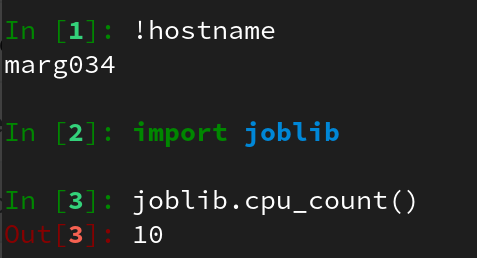
\includegraphics[width=.4\textwidth]{ipython}\\[2em]}

        {\centering  \raisebox{-1ex}{\dangersign[4ex]} Don't forget to release it!\\[1em]}

    \end{frame}

    \begin{frame}[t]{Some more advance info}


        {\bf Other cmd:}\\[.5em]

            \myitem{} \code{sinfo -s}: state of the cluster,\\
            \myitem{} \code{squeue -u \$USER}: current queued job,\\
            \myitem{} \code{sbatch}, \code{salloc}, \code{sacct}, ...: \url{https://slurm.schedmd.com/} \\[1em]

        {\bf Python user tips:}\\[.5em]

        \myitem{} Submitting multiple jobs with \code{submitit} and a \code{concurrent.futures} API: An example of submit script is present \href{https://gitlab.inria.fr/parietal/parietal-wiki/-/blob/master/tutorials/computers/margaret/scripts/submit_script.py}{in the parietal-wiki}
        \\[1em]


        \myitem{} If you have installed \code{conda} on \code{dragostore}, you can access your installation in \code{/data/parietal/store}.

    \end{frame}

\end{document}